%%%%%%%%%%%%%%%%%%%%%%%%%%%%%%%%%%%%%%%%%%%%%%%%%%%%%%%%%%%%%%%%%%%%%%%%%%%%%%
%
% タイトル TeX用テンプレート 
% バージョン 2014-11-8 (Sat) 初版
% 作成者 Kouhei Ito
% 作成場所 野々市市中林 DeuxMKK
% 用途 2段組レポートの作成等
%
%%%%%%%%%%%%%%%%%%%%%%%%%%%%%%%%%%%%%%%%%%%%%%%%%%%%%%%%%%%%%%%%%%%%%%%%%%%%%%%%
%\documentclass[11pt,twocolumn]{jsarticle}
%\documentclass[11pt]{jreport}
%\usepackage[dvipdfmx]{graphicx}
%\usepackage{amsmath,amssymb}
%\usepackage{url}
%\usepackage{nidanfloat}

\documentclass[twocolumn,11pt]{sotsuken_abst}

%% 体裁



%%%%%%%%%%%%%%%%%%%%%%%%%%%%%%%%%%%%%%%%%%%%%%%%%%%%%%%%%%%%%%%%%%%%%%%%%%%%%%%%
\title{超低重心6輪独立懸架ローバーの単眼カメラによる3次元測量}
\author{金沢工業高等専門学校 佐々井翔也,戸澗健,畠中和久(指導教員 伊籐恒平)}
%\date{2016-12-20}
%%%%%%%%%%%%%%%%%%%%%%%%%%%%%%%%%%%%%%%%%%%%%%%%%%%%%%%%%%%%%%%%%%%%%%%%%%%%%%%%
\setcounter{page}{5}
\lhead{}
\chead{}
\rhead{{\sf 16・203}\\{\bf 機械工学科}}
\lfoot{}
\cfoot{{\sf-\ M-\thepage \ -}}
%\rfoot{}
\renewcommand{\headrulewidth}{3pt}
%\renewcommand{\footrulewidth}{1pt}

\begin{document}
%\layout
\maketitle
\thispagestyle{fancy}
\pagestyle{fancy}

\setlength{\baselineskip}{5.6truemm}
\kanjiskip=.07zw plus 3pt minus 3pt
\xkanjiskip=.07zw plus 3pt minus 3pt

%%%%%%%%%%%%%%%%%%%%%%%%%%%%%%%%%%%%%%%%%%%%%%%%%%%%%%%%%%%%%%%%%%%%%%%%%%%%%%%%
\section{緒言}
\subsection{研究の背景}

\subsubsection{安定性の改善}
%そこで今回は走破性の向上を考え,前年度の改善案として低重心化とそれを補佐する懸架装置に注目し,”超低重心6輪独立懸架ローバー”を制作する
前年度,つくばチャレンジで使用したロボットの重心が高かったため,凸凹道やコンクリートなどでロボットが傾きそのまま転倒する恐れがあった.
そのため,前年度の問題点を元に転倒しても走行可能なロボットの開発を試みた.だが,今年度のつくばチャレンジに参加するにあたり,ロボットの高さ制限を満たしかつ転倒しても走行可能な機構の開発ができなかった.
よって今回はロボットの走破性を高めることで,転倒しにくいロボットの開発を行った.
\subsubsection{カメラの移動量とマップの作成}
ロボットが自律走行を行うためには,自身の位置を推定する必要がある.その手段としてローカルマップをグローバルマップに変換する方法が主流である.
一般的にこれを行うためには測域センサーを用いるが,今回は低コストな単眼カメラを用いることにした.また,ローカルマップを生成するために周囲との位置関係を求める必要がある.
カメラでは対象物を写した2枚の画像とそれらの画像間距離から三角測量の原理を用いることで対象物からカメラまでの距離を計測することができる.今回は単眼カメラを用いるため画像間距離はカメラの移動量に等しい.よってカメラの移動量を取得することができれば対象物との位置関係が分かる.

\subsection{研究の目的}
今年度は走破性の向上を考え,前年度の改善案として低重心化とそれを補佐する懸架装置に注目し,”超低重心6輪独立懸架ローバー”を開発する.またカメラの移動量をモーションセンサから得られる位置情報によって取得し,三角測量を行う.これを複数回行い,得られたデータをマップとする.


\section{ハードウェアの概要}
\subsection{ロボットの構成}

今年度のロボットは走行モジュールと制御モジュールで構成されている.また,搭載したセンサを以下の表\ref{tab:op}に示す.


\begin{table}[h]
  \begin{center}
    \caption{ハードウェアの構成}
    \small
  \scalebox{0.85}{
  \begin{tabular}{|c|c|} \hline
    構成要素 & メーカ・型番・スペックなど \\ \hline
    Mian PC & NVIDIA JETSON TK1 \\ \hline
    OS & Ubuntu 14.04 LTS \\ \hline
    camera & Panasonic HX-A1H \\ \hline
    Buttery & KyPOM KT5100 4S 35C \\ \hline
    Motor & MABUCHI MOTOR RS-555VC-5524 \\ \hline
    Motion Sensor & 東京航空計器株式会社 CSM-MG100\\ \hline

  \end{tabular}
  }
    \label{tab:op}
  \end{center}
\end{table}


\subsection{低重心化の実現}
設計した走行モジュールの概要図を図\ref{fig:cad}に示す。図から確認できるように全高がタイヤ直径である190mm内に収まっているため低重心化が達成された.また6輪に付属している懸架装置を図\ref{fig:kenka}に示す.ばねを2本設置することでサスペンションとし,またそれらの取り付け位置を斜めにすることで従来使用されているストラット式と比べて,さらに低重心が可能となった.

\begin{figure}[htp]
 \begin{center}
  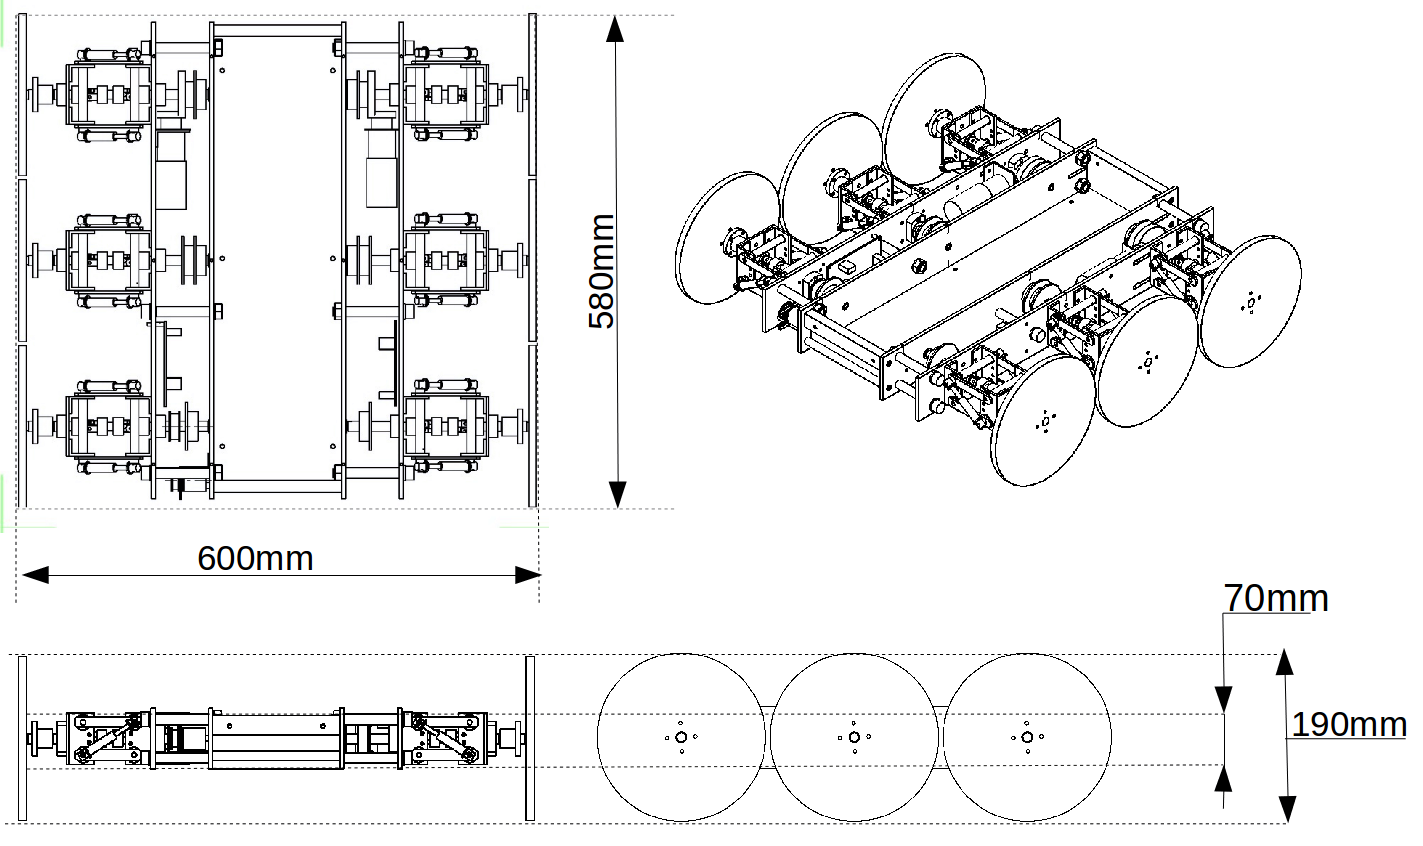
\includegraphics[width=70mm]{image/4.png}
  \caption{走行モジュール}
  \label{fig:cad}%ここに文章中で使用する名前を指定する
 \end{center}
\end{figure}

\begin{figure}[htp]
 \begin{center}
  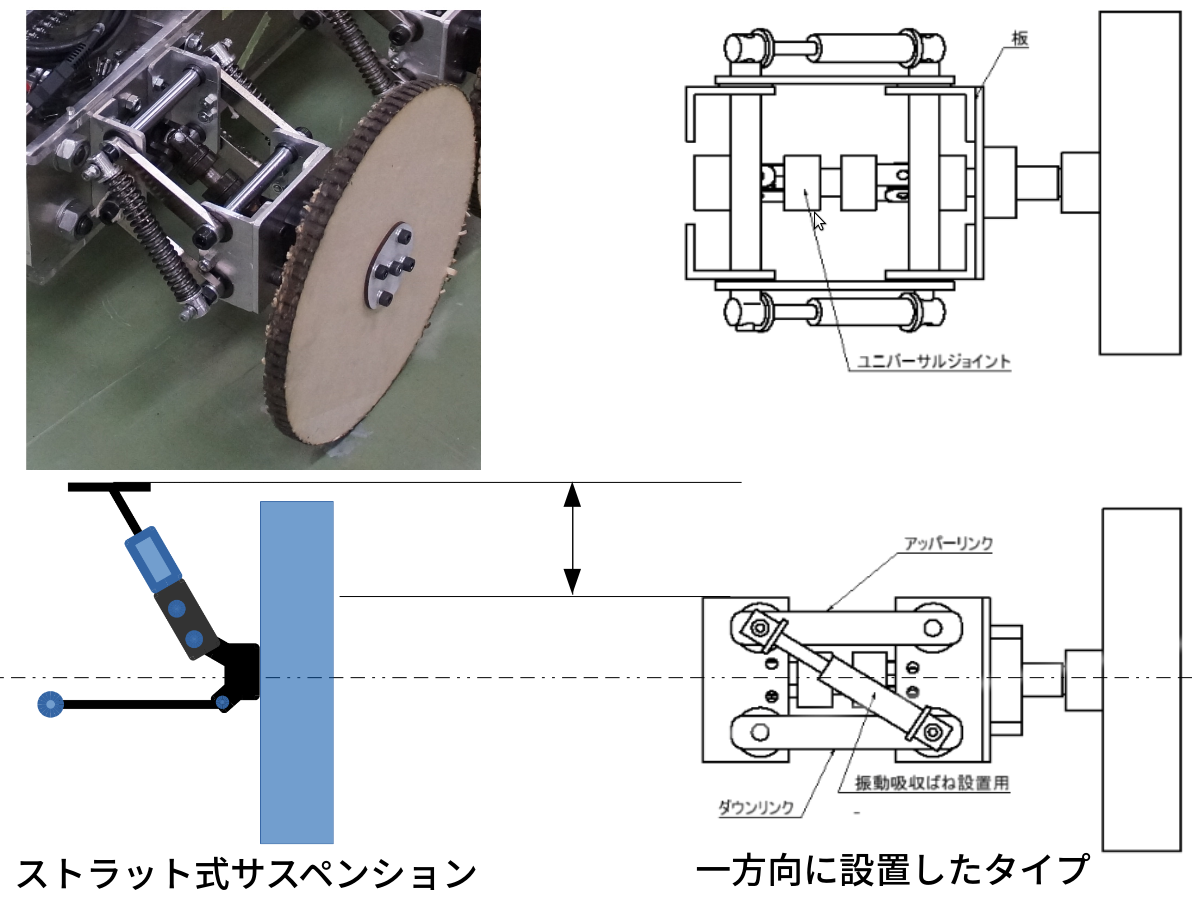
\includegraphics[width=70mm]{image/3.png}
  \caption{懸架装置}
  \label{fig:kenka}%ここに文章中で使用する名前を指定する
 \end{center}
\end{figure}
\subsection{超堤・超壕能力}
今回作成したロボットの性能を調査するため,超堤・超壕実験を行った結果,超堤:110[mm],超壕220[mm]が得られた.

\section{マップ生成}
\subsection{移動量の取得}
カメラの移動量を取得するため,東京航空計器社製のモーションセンサから得られる位置情報を使用する.モーションセンサーを図\ref{fig:motion}に示す.1回目に取得した位置と2回目に取得した位置の
差から移動量を算出する.

\begin{figure}[htp]
 \begin{center}
  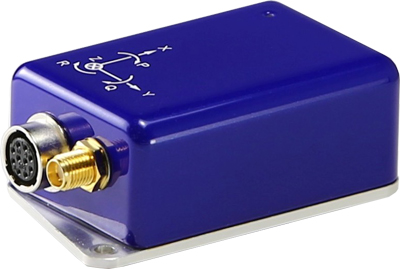
\includegraphics[width=30mm]{image/motion.jpg}
  \caption{モーションセンサー}
  \label{fig:motion}%ここに文章中で使用する名前を指定する
 \end{center}
\end{figure}

\subsection{マップ生成環境}
マップの生成環境を図\ref{fig:map}に示す.天候はカメラ画像に影響の少ないくもりの日,画像間距離を1.4[m]として金沢工業高等専門学校の駐車場付近でマップ生成を行った.ロボットはStart地点から矢印の方向に進み,2回の旋回を経てGoal地点まで走行する.

\subsection{マップ生成}
生成されたマップを図\ref{fig:mapp}に示す.赤い点群はカメラ画像から三角測量によって得られた周囲の位置関係,青い線はカメラ画像から得られたロボットの走行軌跡,黄色い線を実際にロボットが走行した軌跡である.
図より,カメラ画像からマップを生成することができた.
だがカメラ画像から得られたロボットの走行軌跡は1回目の旋回時から,実際にロボットが走行した軌跡と比べて歪んでいることが確認できる.

\begin{figure}[htp]
 \begin{center}
  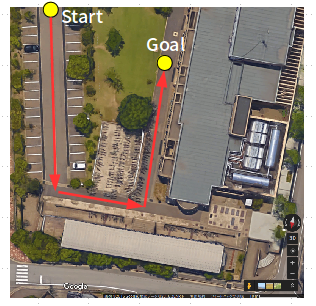
\includegraphics[width=45mm]{image/1.png}
  \caption{マップ生成環境}
  \label{fig:map}%ここに文章中で使用する名前を指定する
 \end{center}
\end{figure}


\begin{figure}[htp]
 \begin{center}
  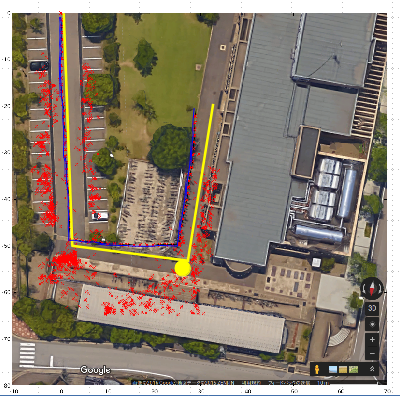
\includegraphics[width=45mm]{image/2.png}
  \caption{生成したマップ}
  \label{fig:mapp}%ここに文章中で使用する名前を指定する
 \end{center}
\end{figure}

\section{結言}
走破性の高いロボットの開発の実現にあたり,つくば市内での走行が問題なく行えたため,走破性の高いロボットの開発は達成したと考える.また移動量の取得とマップ生成の実現にあたり,生成したマップは旋回時に歪むことが確認されたが直線時には問題がなかったため3次元復元技術の基礎は確立できたと考える.

% 参考文献
\begin{thebibliography}{8}
%  \bibitem{harris} LandingProducts, APCPro\nolinebreak pellers,\nolinebreak
%http://www.\linebreak apcprop. com{\slash}v{\slash}index.html,
%2012/8/21
%\bibitem{kyonenn} GPS測位計算プログラム入門,ROS,http://www.enri.go.jp/~fks442/K_MUSEN
\bibitem{ros} Bradski,Kaehler(2012).詳解 OpenCV,株式会社オライリー・ジャパン,433
\bibitem{kyonenn} 理解するためのGPS測位計算プログラム入門,http://www.enri.go.jp/fks442,2016年10月17日%/K_MUSEN
%  \bibitem{koukuu} 中村 資郎:新航空工学講座 第7巻 プロペラ:日本航空技術協会,pp.23-24,1988
%  \bibitem{rikigaku} 加藤 寛一郎,大屋 昭男,柄沢 研治:航空機力学入門,東京大学出版会,pp.32,1982
\end{thebibliography}

%%%%%%%%%%%%%%%%%%%%%%%%%%%%%%%%%%%%%%%%%%%%%%%%%%%%%%%%%%%%%%%%%%%%%%%%%%%%%%%%


\end{document}
